\documentclass[conference]{IEEEtran}

\usepackage{cite}
\usepackage{amsmath,amssymb,amsfonts}
\usepackage{graphicx}
\usepackage{textcomp}
\usepackage{xcolor}
\usepackage{caption}
\usepackage{subcaption}
\usepackage{algorithm}
\usepackage{algpseudocode}
\def\BibTeX{{\rm B\kern-.05em{\sc i\kern-.025em b}\kern-.08em
    T\kern-.1667em\lower.7ex\hbox{E}\kern-.125emX}}

\usepackage[T1]{fontenc}
\usepackage[english]{babel}
\selectlanguage{english}


\usepackage[per-mode=symbol]{siunitx}
\usepackage[nolist,nohyperlinks]{acronym}
\usepackage{wrapfig}

\usepackage{xspace}
\usepackage[hidelinks]{hyperref}
\usepackage[nameinlink, capitalise]{cleveref}

% correct bad hyphenation here
\hyphenation{} %\hyphenation{win-dow net-works com-pu-ter} 

\newcommand{\mycomment}[1]{{\color{red}#1}}
\newcommand{\toremove}[1]{{\color{lightgray}#1}}
\newcommand{\newtext}[1]{{\color{blue}#1}}
%\newcommand{\removable}[1]{{\color{green}#1}}
\newcommand{\removable}[1]{{#1}}
 
\Crefname{figure}{Fig.}{Figs.} %Required by IEEE style
% \renewcommand\figurename{Fig.} %Required by IEEE style (without babel)
\addto\captionsenglish{\renewcommand{\figurename}{Fig.}} %Required by IEEE style (with babel)

\DeclareSIUnit\bpm{bpm}
\DeclareSIUnit\spm{spm}

\begin{acronym}
%   \acro{acronym}[short name]{full name}
    \acro{EEG}{electroencephalogram}
    \acro{MEG}{magnetoencephalogram}
    \acro{AMS}{Auditory-Motor Synchronization}
    \acro{bpm}[\unit{bpm}]{beats per minute}
    \acro{spm}[\unit{spm}]{steps per minute}
\end{acronym}

\newcommand{\ralcoach}{RALCoach\xspace}

%\usepackage[%
 %   text={Extended Abstract},%
 %   scale=0.7,%
 %   color={[rgb]{0.8, 0.1, 0.1}}%
  %  ]{draftwatermark}


\begin{document} 

\title{PortraitNet: Real-time Portrait Segmentation Network for Mobile Device}

\author{
\IEEEauthorblockN{Leonardo Pesce 223100001
}
\IEEEauthorblockN{CIE6004: Image Processing and Computer Vision}
}



\maketitle
\begin{abstract}
    The paper "\textit{PortraitNet: Real-time Portrait Segmentation Network for Mobile Device}" \cite{Zhang2019PortraitNetRP} introduces PortraitNet, a real-time portrait segmentation model designed for mobile devices. It utilizes a lightweight U-shape architecture with two auxiliary losses during training, specifically the boundary loss and consistency constraint loss, to improve accuracy and robustness. PortraitNet outperforms existing methods in accuracy and efficiency, particularly in generating sharper boundaries and handling challenging lighting conditions. Additionally, it can process 224 × 224 RGB images at 30 FPS on an iPhone 7 in real-time.

\end{abstract}
\section{Introduction}
The paper discusses the growing importance of real-time portrait segmentation, driven by the demand for mobile applications that enable background editing of portrait images. It highlights the challenges posed by the unique characteristics of portrait images, such as the need for precise segmentation in the presence of ambiguous boundaries and varying illumination conditions. Existing methods have prioritized accuracy over efficiency, making them unsuitable for real-time mobile applications.

To address these challenges, the authors propose PortraitNet, a specialized convolutional neural network designed for real-time portrait segmentation on mobile devices. PortraitNet utilizes a specific network architecture with a 32× down-sampling rate to enhance efficiency and employs a U-shape architecture for better segmentation. The network is trained using auxiliary losses, including a boundary loss to improve boundary accuracy and a consistency constraint loss to enhance robustness under varying illumination.

The results demonstrate that PortraitNet achieves high accuracy, with 96.62\% accuracy on the EG1800 dataset and 93.43\% on the SupervisePortrait dataset. Furthermore, it can process images at 30 frames per second on an iPhone 7 with an input size of 224 × 224, making it suitable for real-time mobile portrait segmentation.


\section{Method}
\subsection{Model Structure}
Let's now have a look at the model implemented in the paper. The model is based on the MobileNet-v2 \cite{DBLP:journals/corr/abs-1801-04381}, which is an architecture specifically designed for mobile devices (low computational power). The MobileNetV2 design employs an inverted residual structure, which differs from traditional residual models by utilizing slender bottleneck layers for both input and output within the residual block. Instead of expanded representations in the input, MobileNetV2 employs lightweight depthwise convolutions to filter features in the intermediate expansion layer. 

The structure is U-shape with a x32 downsampling in the encoder phase that combined with the residual architecture extracts global and spatial information about the image.


\subsection{Auxiliary Losses}
To make up for the lower complexity of the model (since it needs to run in real-time) two auxiliary losses are introduced.

\subsubsection{Boundary Loss}
Given that, portrait segmentation needs sharper edges and that the edge represents less than 10\% of the labeled dataset we use the focal loss to balance this fact. Focal loss $L_e$ is combined with cross-entropy loss $L_m$ in the following way:

\begin{equation}
    L=L_m + \lambda L_e
\end{equation}

\begin{equation}
    L_m = - \sum_{i=1}^{n}(y_ilog(p_i)+(1-y_i)log(1-p_i))
\end{equation}

\begin{equation}
    L_e = - \sum_{i=1}^{n}(1-p_i)^\gamma y_ilog(p_i)) + p_i^{\gamma}(1-y_i)log(1-p_i))
\end{equation}

Where $\gamma$ is the weight of the boundary loss, and the probability $p_i$ is computed as 

\begin{equation}
    p_i(z_j)=\frac{e^{z_j}}{\sum_{k=1}^Ke^{z_k}}
\end{equation}


\subsubsection{Consistency Constraint Loss}
In general, in a segmentation process, hard labels (binary labels) are used. Given our complexity requirements, since it has been shown that for small models soft labels help in the training process, a new method to generate soft labels is proposed (usually generating soft labels requires a teacher model that needs extensive training). 
Given an input $A$ a second input $A'$ is generated simply by a texture enhancement transformation (change in brightness, contrast, sharpness, noise...).
At this point, both images are passed through the model obtaining the output $B$ and $B'$. $B'$ is worse than $B$ because it was generated by $A'$, a lower quality version of $A$. In the end, $B$ is used as a higher quality soft label for $B'$ and the KL-divergence is used to compute the loss between the two:

\begin{equation}
    L=L_M'+\alpha\times L_c 
\end{equation}

\begin{equation}
    L_c = \frac{1}{n}\sum_{i=1}^n q_i \times log\frac{q_i}{q_i'} \times T^2
\end{equation}

\begin{align}
\begin{split}
    L_m' = &- \sum_{i=1}^{n}(y_ilog(p_i)+(1-y_i)log(1-p_i)) \\ 
    &- \sum_{i=1}^{n}(y_ilog(p_i')+(1-y_i)log(1-p_i'))
\end{split}
\end{align}

Where $\alpha$ is used to balance the two losses, $T$ to smooth the output, $p_i$ and $p_i'$ are:

\begin{equation}
    p_i(z_j)=\frac{e^{z_j}}{\sum_{k=1}^Ke^{z_k}}
    \qquad
    p_i'(z_j')=\frac{e^{z_j'}}{\sum_{k=1}^Ke^{z_k'}}
\end{equation}

and $q_i$ and $q_i'$ are:

\begin{equation}
    p_i(z_j)=\frac{e^{\frac{z_j}{T}}}{\sum_{k=1}^Ke^{\frac{z_j'}{T}}}
    \qquad
    p_i'(z_j')=\frac{e^{\frac{z_j'}{T}}}{\sum_{k=1}^Ke^{\frac{z_k'}{T}}}
\end{equation}

Adding this loss results in higher accuracy and robustness under different lighting conditions.
\section{Results}
The model trained for 1000 epochs with a batchsize of 64, a learning rate of 0.001, momentum of 0.9 and weight decay of 0.0005.
We now run our model on the dataset provided EG1800 and test its accuracy and results. 
For every example there are 4 images, the first and the third contain the predicted mask and edge of the person, while the second and the fourth contains the real mask and edge.


\begin{figure}[H]
    \centering
    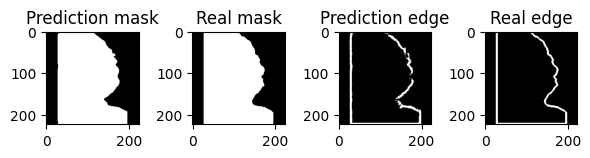
\includegraphics[width=0.98\linewidth]{media/download (1).png}
    \caption{example 1}
    \label{fig:enter-label}
\end{figure}

\begin{figure}[H]
    \centering
    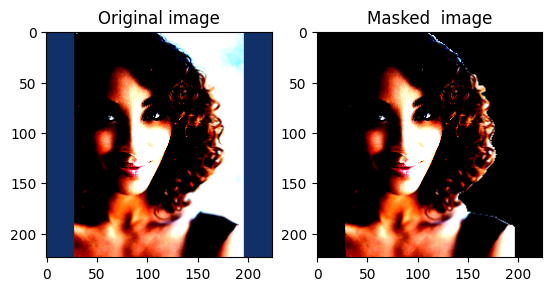
\includegraphics[width=0.98\linewidth]{media/download (6).png}
    \caption{mask result of example 1}
    \label{fig:enter-label}
\end{figure}

\begin{figure}[H]
    \centering
    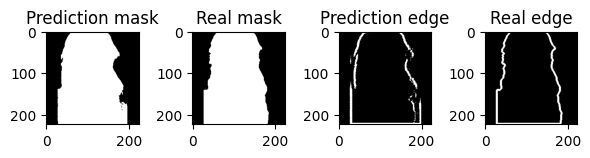
\includegraphics[width=0.98\linewidth]{media/download (2).png}
    \caption{example 2}
    \label{fig:enter-label}
\end{figure}

\begin{figure}[H]
    \centering
    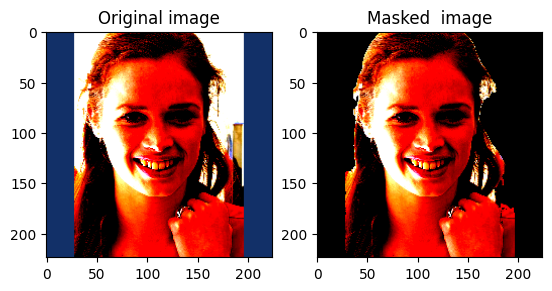
\includegraphics[width=0.98\linewidth]{media/download (7).png}
    \caption{mask result of example 2}
    \label{fig:enter-label}
\end{figure}

\begin{figure}[H]
    \centering
    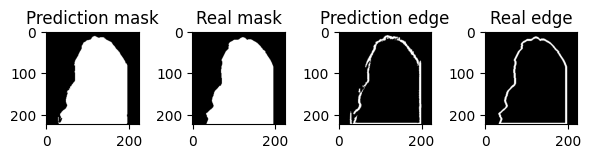
\includegraphics[width=0.98\linewidth]{media/download (3).png}
    \caption{example 3}
    \label{fig:enter-label}
\end{figure}

\begin{figure}[H]
    \centering
    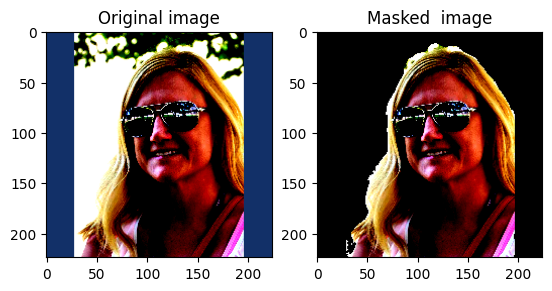
\includegraphics[width=0.98\linewidth]{media/download (8).png}
    \caption{mask result of example 3}
    \label{fig:enter-label}
\end{figure}

\begin{figure}[H]
    \centering
    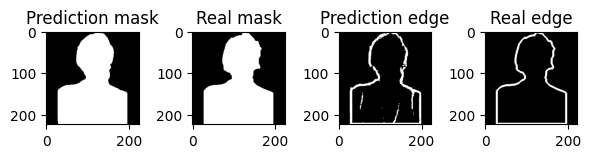
\includegraphics[width=0.98\linewidth]{media/download (4).png}
    \caption{example 4}
    \label{fig:enter-label}
\end{figure}

\begin{figure}[H]
    \centering
    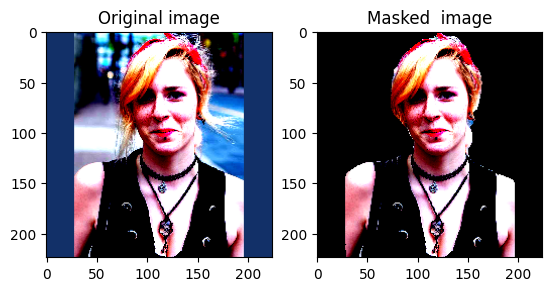
\includegraphics[width=0.98\linewidth]{media/download (9).png}
    \caption{mask result of example 4}
    \label{fig:enter-label}
\end{figure}

\begin{figure}[H]
    \centering
    \includegraphics[width=0.98\linewidth]{media/download(5).png}
    \caption{example 5}
    \label{fig:enter-label}
\end{figure}

\begin{figure}[H]
    \centering
    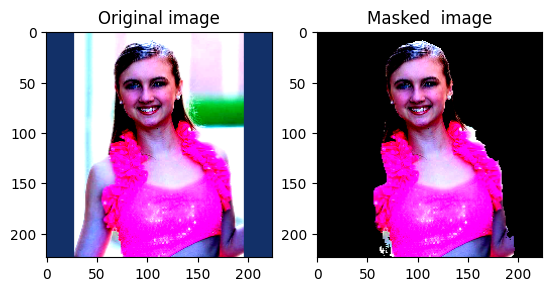
\includegraphics[width=0.98\linewidth]{media/download (10).png}
    \caption{mask result of example 5}
    \label{fig:enter-label}
\end{figure}

We can see that the model provides very good visual results, given the smaller complexity in respect to other model.  
\section{Conclusions}

The paper discusses the creation of a light and fast neural network architecture based on MobileNet-v2 to segment people inside picture (with a target on mobile devices).

\bibliographystyle{IEEEtran}
\bibliography{export}

\end{document}

% EXAMPLE OF PSEUDOCODE
\begin{algorithm}[H]
    \caption{pseudocode for illumination change}\label{alg:cap}
    \begin{algorithmic}
        \State compute matrix A (Discrete Poisson equation)
        \For{number of color channels in picture}
        \State change the image to the log domain
        \State compute $\nabla f$ and $|\nabla f|$
        \State compute $\alpha$ and $\beta$
        \State $\mathbf{v} = \alpha^\beta|\nabla f^*|^{-\beta}\nabla f^*$
        \State construct vector b with $\mathbf{v}$
        \State compute the solution to $Ax=b$
        \State revert the image to the original domain
        \EndFor
        \State reconstruct the image from the solutions
    \end{algorithmic}
\end{algorithm}




%EXAMPLE OF MULTIPLE (3) IMAGE IN LINE (HALF COLUMN)
\begin{figure}[H]
    \centering
    \begin{subfigure}{0.32\linewidth}
        \centering
        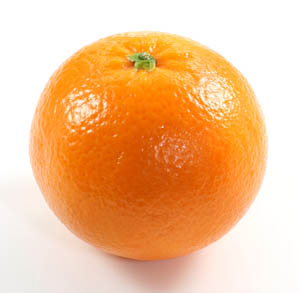
\includegraphics[width=0.98\linewidth]{media/illumination_changes/source_light.jpg}
        \caption{source image}
        \label{fig:enter-label}
    \end{subfigure}
    \hfill
    \begin{subfigure}{0.32\linewidth}
        \centering
        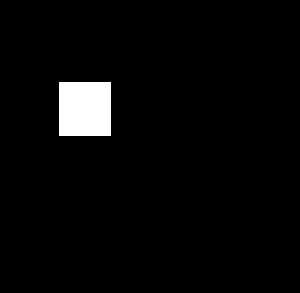
\includegraphics[width=0.98\linewidth]{media/illumination_changes/mask_light.jpg}
        \caption{mask image}
        \label{fig:enter-label}
    \end{subfigure}
    \hfill
    \begin{subfigure}{0.32\linewidth}
        \centering
        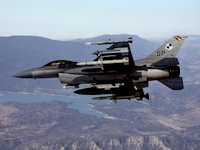
\includegraphics[width=0.98\linewidth]{media/illumination_changes/result.png}
        \caption{result image}
        \label{fig:enter-label}
    \end{subfigure}
    \label{fig2}
\end{figure}


